% Poster design after an idea from
% http://wwwalt.tp4.ruhr-uni-bochum.de/SoftwareDocs/poster/poster_doc.html
\documentclass[a0,portrait]{a0poster}
\usepackage[T1]{fontenc}
\usepackage[utf8]{inputenc}
% Use Times font...
\usepackage{times}
% ... but Computer Modern typewriter font
\renewcommand{\ttdefault}{lmtt}
%\usepackage{lmodern}
\usepackage{amsfonts}

\usepackage{paths}

\usepackage[svgnames]{xcolor}

%\usepackage{footmisc}
\usepackage{alltt}
\usepackage{amsthm}
\usepackage{amsmath}
\usepackage{ccaption}
\usepackage{float}
\usepackage{graphicx}
\usepackage{hyperref}
\usepackage{listings}
\usepackage{multicol}
\usepackage{pgflibraryarrows}
\usepackage{sectsty}
\usepackage{tikz}
\usepackage{wrapfig}

\let\RealRightarrow=\Rightarrow
\usepackage{marvosym}
\renewcommand{\Rightarrow}{\RealRightarrow}
\usepackage{wasysym}

\lstset{basicstyle=\ttfamily\normalsize,basewidth=0.5em,aboveskip=-2ex,belowskip=-2ex}

% KWARC macros
\usepackage{acronyms,misc-macros,semantic-markup}

% some colors
\definecolor{light-yellow}{rgb}{1,1,0.8} 
\definecolor{dark-blue}{rgb}{0.1,0,0.7}

\newcommand{\SemColor}[1]{\textcolor{DarkGreen}{#1}}
\newcommand{\CollColor}[1]{\textcolor{Maroon}{#1}}
\newcommand{\SciColor}[1]{\textcolor{DarkBlue}{#1}}
\newcommand{\SvcColor}[1]{\textcolor{SaddleBrown}{#1}}

% font and other styles
\def\defaulttextfont{\Large}
\sectionfont{\huge}
\subsectionfont{\LARGE}
%\setlength{\parskip}{-10pt}
\setlength{\columnsep}{1.9cm}
\setlength{\columnseprule}{1pt}
%\newcommand{\footnotelayout}{\normalsize}

% TikZ styles
\tikzstyle{default}=[very thick,font=\sffamily,>=triangle 60]
\tikzstyle concept=[font=\sffamily\bfseries\large,draw,minimum height=3.5ex,rounded corners]

% local macros
\def\ExprColor#1{#1}
\def\ElisColor#1{#1}
\def\llquote#1{\ensuremath{\langle\kern-.25em\langle\hbox{\sl{#1}}\rangle\kern-.25em\rangle}}
\def\mod{{\rm{mod}}}
\def\pres#1#2{\overline{#1}^{#2}}  
\def\lden{[\kern-.15em[}\def\rden{]\kern-.15em]}
\def\defemph#1{{\bf{#1}}}
\def\imarg#1#2{\fbox{\ensuremath{\left.#1\right|_{#2}}}}
\def\fimarg#1#2#3{\fbox{\ensuremath{\left.#1\right|_{#2}^{#3}}}}
\def\recu#1{#1}%should be changed to notation for <recurse precedence="#1"/>, maybe a circle around p

\newcommand{\corresponds}{\mathrel{\widehat{=}}}
\newenvironment{authorbox}[1]{\begin{minipage}[c]{#1}\centering\Large\bf}{\end{minipage}}
\newcommand{\logobox}[2]{\begin{minipage}[c]{#1}\centering\includegraphics[width=\textwidth]{#2}\end{minipage}}
\newcommand{\yellowbox}[1]{%
    \renewcommand{\rmdefault}{lmr}%
    \setlength{\fboxrule}{0.1cm}%
    \setlength{\fboxsep}{.5cm}%
    {\begin{center}%
    \fcolorbox{black}{light-yellow}%
    {\parbox{0.9\textwidth}%
    {\vspace{0.5cm} \bf \Large #1
    \vspace{0.5cm}}}\end{center}}%
    \renewcommand{\rmdefault}{ptm}}
\newcommand{\colored}[1]{\textcolor{DarkRed}{#1}}
\newcommand{\bsl}{\symbol{'134}}
% Hyphenation
\hyphenation{Math-ML}

\begin{document}

\begin{center}
  % FIRST LOGO
  \begin{minipage}[c]{0.19\textwidth}\centering\includegraphics[width=\textwidth]{Jacobs_LOGO_RGB}\end{minipage}%
  % HEADING
  \begin{minipage}[c]{0.62\textwidth} 
    \begin{center}
      {\veryHuge \bf
        \begin{tabular}[t]{c}
          Presenting Mathematical Content\\
          with Flexible Elisions
        \end{tabular}}\\
      \vspace{1cm}
      \begin{authorbox}{\textwidth}
        Michael Kohlhase \texttt{<m.kohlhase>}, Christoph Lange
        \texttt{<ch.lange>}, Florian Rabe \texttt{<f.rabe>}\\[.5cm]
      Knowledge Adaptation and Reasoning for Content, Computer Science\\
        Jacobs University, Bremen, Germany \texttt{<...@jacobs-university.de>}
      \end{authorbox}
    \end{center}
\end{minipage}%
  % SECOND LOGO
  \begin{minipage}[c]{0.19\textwidth}\centering\includegraphics[width=.7\textwidth]{kwarc}\end{minipage}%
\end{center}
\vspace{0.5cm} \yellowbox{Mathematicians frequently elide brackets or symbols in
  formulae to concentrate on essential facts and to avoid distracting
  experienced mathematicians with notation that can easily be deduced from
  context.  We propose a content dictionary format for content markup languages
  like Content {\mathml} or {\openmath} that supports flexary mixfix operators
  and is capable of handling flexible elisions.}  \vspace{0.5cm} \defaulttextfont
\begin{multicols}{2}
\raggedright

\section*{Presentation as Composition and Elision}
\label{sec:intro}

\begin{minipage}[t]{.36\linewidth}
  {\raggedright
  \begin{enumerate}
    \setcounter{enumi}{-1}
  \item Content representations (variables, symbols, applications, binders)
  \end{enumerate}}
\begin{center}
  \begin{tikzpicture}[xscale=4,yscale=3.5,font=\LARGE]
    \node[circle,fill=green!20] (top) at (1,2) {@};
    \node[draw] (plus) at (0,1) {\textcolor{blue!75}{plus}};
    \node[circle,fill=red!20] (mid) at (1,1) {@};
    \node[draw] (y) at (2,1) {y};
    \node[draw] (mult) at (0,0) {\textcolor{violet}{times}};
    \node[draw] (a) at (1,0) {a};
    \node[draw] (x) at (2,0) {x};
    \draw(top) -- (plus);
    \draw(top) -- (mid);
    \draw(top) -- (y);
    \draw(mid) -- (mult);
    \draw(mid) -- (a);
    \draw(mid) -- (x);
  \end{tikzpicture}
\end{center}
\end{minipage}\hspace{.01\linewidth}%
\begin{minipage}[t]{.30\linewidth}
  {\raggedright
  \begin{enumerate}
  \item 2D \emph{composition} of presentations\newline (formula tree\newline $\to$
    layout tree)
  \end{enumerate}}
\begin{center}
  \begin{tikzpicture}[scale=2,font=\huge]
    \fill[green!20] (-0.2,-0.2) rectangle +(3.4,1.4);
    \draw (0,0) rectangle +(1,1);
    \node at (1.5,0.5) {\textcolor{blue!75}{\textbf{+}}};
    \draw (2,0) rectangle +(1,1);
    \node (y) at (2.5,0.5) {$y$};
    \node[rectangle,draw,dashed,fill=red!20] (x) at (0.5,-1.5) {$a\textcolor{violet}{\cdot}x$};
    \draw[dashed] (0,0) -- (x.north west);
    \draw[dashed] (1,0) -- (x.north east);
  \end{tikzpicture}
\end{center}
\end{minipage}\hspace{.01\linewidth}%
\begin{minipage}[t]{.30\linewidth}
  {\raggedright
  \begin{enumerate}
    \setcounter{enumi}{1}
  \item \emph{elision} of parts that can be deduced from the context
  \end{enumerate}}
\begin{center}
  \begin{tikzpicture}[scale=2.5,font=\huge]
    \node (1) at (0,2) {\colorbox{green!20}{$\text{\colorbox{red!20}{$(a\textcolor{violet}{\cdot}x)$}}\textcolor{blue!75}{+}y$}};
    \node (2) at (0,0) {\colorbox{green!20}{$\text{\colorbox{red!20}{$ax$}}\textcolor{blue!75}{+}y$}};
    \draw[->,>=triangle 60] (1) -- (2);
  \end{tikzpicture}
\end{center}
\end{minipage}\\
%%% (1) CURRENTLY WELL-UNDERSTOOD, (2) MUCH LESS SO.

\section*{Characteristics of Mathematical Symbols}
\label{sec:charac}

\begin{minipage}[t]{.55\linewidth}
  \raggedright
  \begin{description}
  \item[fixity:] pre-/post-/in-/mixfix
  \item[brackets:] left and right, mostly round
  \item[associativity:] fully/left/right
  \end{description}
\end{minipage}%
\begin{minipage}[t]{.4\linewidth}
  \raggedright
  \Lightning{} These are not real \emph{brackets}:
  \[
  ]a;b],\;\{x\in\mathbb{N}|x>5\},\;\binom{n}{k},\ldots
  \]
\end{minipage}
\section*{Notation Definitions: symbol- vs.\ template-based}
\label{sec:notdef}

\begin{minipage}[t]{.31\linewidth}
  \raggedright
{\small
\begin{alltt}
<presentation\hfill\(\text{\rm ({\omdoc} 1.2, '06)}\)
 \textcolor{DarkRed!75}{for="power" theory="arith1"}
 role="\textcolor{violet!75}{application}" \textcolor{DarkGreen!75}{class="1"}>
  <style format="\textcolor{blue!75}{TeX}">
    \textcolor{DarkGoldenrod!75}{<recurse select="*[2]"/>}
    <text>\textcolor{DarkSlateGray!75}{^\{}</text>
    \textcolor{DarkGoldenrod!75}{<recurse select="*[3]/>}
    <text>\textcolor{DarkSlateGray!75}{\}}</text>
  </style>
<presentation>
\end{alltt}}
\end{minipage}\hspace{.02\linewidth}%
\begin{minipage}[t]{.38\linewidth}
  \raggedright
{\small
\begin{alltt}
<Notation>\hfill\(\text{\rm (Naylor \& Watt '01)}\)
  <version \textcolor{DarkGreen!75}{style="1"}>
    \textcolor{blue!75}{<tex>}\textcolor{DarkGoldenrod!75}{\bsl{}arg\{a1\}\{n\}}\textcolor{DarkSlateGray!75}{^\{}\textcolor{DarkGoldenrod!75}{\bsl{}arg\{a2\}\{m\}}\textcolor{DarkSlateGray!75}{\}}\textcolor{blue!75}{</tex>}
  </version>
  <semantic-template>
    \textcolor{violet!75}{<OMA>}\textcolor{DarkRed!75}{<OMS cd="power" name="arith1"/>}
      \textcolor{DarkGoldenrod!75}{<OMV name="n" id="a1/>}
      \textcolor{DarkGoldenrod!75}{<OMV name="n" id="a2/>}
    \textcolor{violet!75}{</OMA>}
  </semantic-template>
</Notation>
\end{alltt}}
\end{minipage}\hspace{.02\linewidth}%
\begin{minipage}[t]{.25\linewidth}
  \raggedright
  \begin{itemize}
  \item easier than XSLT
  \item roughly equivalent
  \end{itemize}
\end{minipage}

\section*{A Mixfix Presentation Model for Flexary Terms}
\label{sec:mixfix}

\begin{minipage}{.64\linewidth}
\[f=w_0\imarg{p_1}{\pi_1}w_1\imarg{p_2}{\pi_2}\ldots\imarg{p_n}{\pi_n}w_n:p\]
\end{minipage}%
\begin{minipage}{.34\linewidth}
  \raggedright
  (Paulson '05, {\isabelle})
\end{minipage}\\[1ex]

$w_i$: strings in the output language, $p$: output precedence, boxes: argument
specifications (rendered recursively), $p_i$: input precedences.  Argument is bracketed when its operator binds weaker than the enclosing operator.

\begin{minipage}{.64\linewidth}
  \[\imarg{p}{1}\text{\ensuremath{\backslash}vdash\_}\left\{\imarg{p}{2}\right\}\;\imarg{p}{3}\colon\imarg{p}{4}:p\]
\end{minipage}%
\begin{minipage}{.34\linewidth}
  \centering
\textit{Typing judgment ($\Gamma\vdash_\Sigma t\colon\alpha$) in \LaTeX}
\end{minipage}\\[1ex]

{\openmath} and Content {\mathml} require \ExprColor{flexible arities}!\\

\begin{minipage}{.64\linewidth}
\[\fimarg{\times:\recu{p-1}}{1}{n-1}\to\imarg{\recu{p}}{n}:p\]
\end{minipage}%
\begin{minipage}{.34\linewidth}
  \centering
\textit{The space of $n$-ary functions}
\end{minipage}\\[1ex]


\section*{Flexible Elisions}
\label{sec:elisions}

Elision desired for redundant brackets, default or inferable argument values.
\[ax+y=(a\cdot x)+y\qquad\log x=\log_{10}x\qquad\lden t\rden=\lden t\rden_{\cal M}^\phi, \qquad\ldots\]
Flexible elisions serve experts and beginners.
\begin{itemize}
\item \ElisColor{\emph{visibility levels}} (for brackets: \emph{precedence
    difference}) per \ElisColor{\emph{elision group}}, user can choose
  visibility threshold per group
\item static output format (e.\,g.\ dead tree): choice at generation
\item dynamic output format: elision annotations; interactive choice
\end{itemize}

\begin{center}
  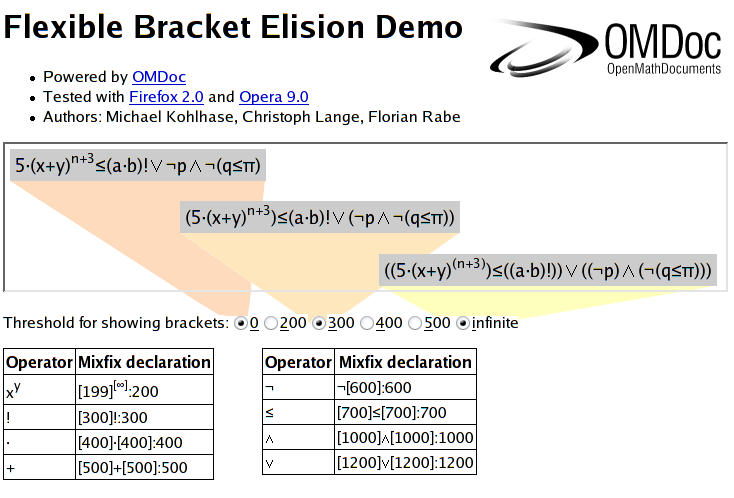
\includegraphics[width=.84\linewidth]{demo-shot}
\end{center}
\section*{The Flexary Mixfix Model in a CD Format}
\label{sec:omdoc2}

Made {\omdoc} more powerful, deprecated embedded XSLT.  Syntactic sugar for
fixities and format-independent settings.

How is notation definition for symbol determined? -- Look up (1) exact match,
(2) ``default'' presentation.  Choice among $\ge 1$ presentations is non-trivial
($\to$ Kohlhase/Müller/Müller '07).

\begin{minipage}[t]{.6\linewidth}
  \raggedright
  {\normalsize Example: the typing jugdment $\Gamma\vdash_\Sigma t:T$ in
    {\LaTeX}}
  {\small
\begin{alltt}
<symbol \textcolor{DarkRed!75}{name="typing-judgment"} \textcolor{violet!75}{role="application"}/>
<presentation \textcolor{DarkRed!75}{for="#typing-judgment"}
 \textcolor{violet!75}{role="application"} format="latex">
  \textcolor{DarkGreen!75}{<map begin="1"/>}
  <text>\textcolor{DarkSlateGray!75}{\bsl{}vdash_\{}</text>\textcolor{DarkGoldenrod!75}{<map begin="2"/>}<text>\textcolor{DarkSlateGray!75}{\}}</text>
  \textcolor{blue!75}{<map begin="3"/>}
  <text>\textcolor{DarkSlateGray!75}{:}</text>
  \textcolor{DeepPink!75}{<map begin="4"/>}
</presentation>
\end{alltt}}
\end{minipage}\hspace{.02\linewidth}%
\begin{minipage}[t]{.35\linewidth}
  \raggedright
  {\normalsize Input:}
  {\small
\begin{alltt}
\textcolor{violet!75}{<OMA>}
  \textcolor{DarkRed!75}{<OMS name="typing-judgment" cd="typ"/>}
  \textcolor{DarkGreen!75}{<OMS name="emptyset" cd="sets"/>}
  \textcolor{DarkGoldenrod!75}{<OMV name="\(\Sigma\)"/>}
  \textcolor{blue!75}{<OMS name="true" cd="boolean"/>}
  \textcolor{DeepPink!75}{<OMS name="Boolean" cd="boolean"/>}
\textcolor{violet!75}{</OMA>}
\end{alltt}}
{\normalsize Output:}
{\small
\begin{alltt}
\textcolor{DarkGreen!75}{\bsl{}emptyset}\textcolor{DarkSlateGray!75}{\bsl{}vdash_\{}\textcolor{DarkGoldenrod!75}{\(\textcolor{DarkGoldenrod!75}{\Sigma}\)}\textcolor{DarkSlateGray!75}{\}}
  \textcolor{blue!75}{\bsl{}mathit\{true\}}\textcolor{DarkSlateGray!75}{:}\textcolor{DeepPink!75}{\bsl{}mathit\{Boolean\}}
\end{alltt}}

{\normalsize
Rendered: }$\textcolor{DarkGreen!75}{\emptyset}\mathop{\textcolor{DarkSlateGray!75}{\vdash}}_{\textcolor{DarkGoldenrod!75}{\Sigma}}\textcolor{blue!75}{\mathit{true}}\mathop{\textcolor{DarkSlateGray!75}{:}}\textcolor{DeepPink!75}{\mathit{Boolean}}$
\end{minipage}\\[1ex]

Flexary notation and multiple output formats:
\begin{minipage}[t]{.6\linewidth} {\small
\begin{alltt}
<symbol \textcolor{DarkRed!75}{name="times"} \textcolor{violet!75}{role="application"}/>
<presentation \textcolor{DarkRed!75}{for="#times"} \textcolor{DeepPink!75}{role="constant"} \textcolor[HTML]{3232B1}{format="ascii"}>
  <text>*</text>
</presentation>
<presentation \textcolor{DarkRed!75}{for="#times"} \textcolor{DeepPink!75}{role="constant"} \textcolor[HTML]{3232B1}{format="latex"}>
  <text>\bsl{}ast</text>
</presentation>
<presentation \textcolor{DarkRed!75}{for="#times"} \textcolor{violet!75}{role="application"}
 precedence="400" \textcolor[HTML]{3232B1}{format="ascii latex"}>
  \textcolor{DarkGoldenrod!75}{<text egroup="lbrack">(</text>}
  \textcolor{DarkGreen!75}{<map begin="1" end="-1">}
    <separator>\textcolor{DeepPink!75}{<map begin="0"/>}</separator>
    \textcolor{DarkGreen!75}{<recurse precedence="400"/>}
  \textcolor{DarkGreen!75}{</map>}
  \textcolor{DarkGoldenrod!75}{<text egroup="rbrack">)</text>}
</presentation>
\end{alltt}}
\end{minipage}\hspace{.02\linewidth}%
\begin{minipage}[t]{.35\linewidth}
  {\normalsize Input:}
  {\normalsize
\begin{alltt}
<apply><power/>
  \textcolor{violet!75}{<apply>}\textcolor{DarkRed!75}{<times/>}
    \textcolor{DarkGreen!75}{<ci>x</ci><ci>y</ci>}
  \textcolor{violet!75}{</apply>}
  <cn>2</cn>
</apply>
\end{alltt}}
      {\normalsize Output:
      \begin{description}
      \item[{\textcolor[HTML]{3232B1}{\LaTeX:}}] $\textcolor{DarkGoldenrod!75}{(}\textcolor{DarkGreen!75}{a}\mathop{\textcolor{blue!75}{\ast}}\textcolor{DarkGreen!75}{b}\textcolor{DarkGoldenrod!75}{)}^2$
      \item[{\textcolor[HTML]{3232B1}{ASCII:}}] \begin{alltt}\textcolor{DarkGoldenrod!75}{(}\textcolor{DarkGreen!75}{a}\textcolor{blue!75}{*}\textcolor{DarkGreen!75}{b}\textcolor{DarkGoldenrod!75}{)}^2\end{alltt}
      \end{description}}
    \end{minipage}\\[1ex]

Bracket elision in Presentation {\mathml}:
{\small
\begin{alltt}
<presentation \textcolor{DarkRed!75}{for="#plus"} precedence="500">...</presentation>
<presentation \textcolor{DarkRed!75}{for="#times"} precedence="400">
  \textcolor{DarkGoldenrod!75}{<element name="mo" egroup="lbrack"><text>(</text></element>}
  ...
</presentation>
\end{alltt}}
    \begin{minipage}{.45\linewidth}
      {\normalsize Input:
\begin{alltt}
<OMA>
  \textcolor{DarkRed!75}{<OMS name="plus" cd="arith1"/>}
  <OMA>
    \textcolor{DarkRed!75}{<OMS name="times" cd="arith1"/>}
    <OMV name="a"/>
    <OMV name="x"/>
  </OMA>
  <OMV name="y"/>
</OMA>
\end{alltt}}
    \end{minipage}%
    \begin{minipage}{.45\linewidth}
      {\normalsize Output:
\begin{alltt}
<mrow>
  <mrow>
    \textcolor{DarkGoldenrod!75}{<mo style="display:none"
     omdoc:elevel="100">(</mo>}
    <mi>a</mi>\textcolor{DarkRed!75}{<mo>\(\cdot\)</mo>}<mi>x</mi>
    \textcolor{DarkGoldenrod!75}{<mo style="display:none"
     omdoc:elevel="100">)</mo>}
  </mrow>
  \textcolor{DarkRed!75}{<mo>+</mo>}<mi>y</mi>
</mrow>
\end{alltt}}
    \end{minipage}
\end{multicols}
\vspace{1cm} \yellowbox{Our approach is knowledge-based, extensible, adaptive,
  mathematical, and efficient.  We propose a manageable declarative notation for
  content dictionaries that allows for generating interactive human-oriented
  presentations, adaptable to the level of experience of the reader.  We propose
  this notation for the {\mathml} 3 recommendation.}
\end{document}

% vim:tw=90:autoindent:

% LocalWords:  Wiki iub Lange Universität SWiM wiki emat ics ath uments OMA cd
% LocalWords:  arith OMV nat sion Wikis OMDoc's da aa taxonomics nt expn expl
% LocalWords:  susp Schaffert et al
